\section{Ranked Group Fairness Verification and Model Adjustment}
To verify ranked group fairness efficiently in time $O(k)$, a pre-computed data structure of the inverse multinomial CDF with parameters $k, p_G$ and $ \alpha $ can be used.
%
The inverse CDF specifies value of a random variable such that the probability of the variable being less than or equal to that value equals a given probability (in our case $p_G$).
%
\subsection{Verifying ranked group fairness for a single protected group. }
%
For binomial distributions, i.e. where only one protected and one non-protected group is present, the inverse CDF is called the quantile function.
%
Table~\ref{tbl:ranked_group_fairness_table} shows an example of such a pre-computed data structure with different $ k $ and $ p $, using $\alpha=0.1$.
%
For instance, for $p=0.5$ we see that at least 1 candidate from the protected group is needed in the top 4 positions, and 2 protected candidates in the top 7 positions.

\begin{table}[t!]
	\caption{Example values of $m_{\alpha,p}(k)$, the minimum number of candidates in the protected group that must appear in the top $k$ positions to pass the ranked group fairness criteria with $\alpha=0.1$ in a binomial setting.}
	\vspace{-3mm}
	\label{tbl:ranked_group_fairness_table}
	\small\begin{tabular}{r|cccccccccccc}
		\diaghead{some text}%
		{p}{k}&
		% & \multicolumn{10}{c}{k} \\
		1 & 2 & 3 & 4 & 5 & 6 & 7 & 8 & 9 & 10 & 11 & 12 \\ \midrule
		0.1      & 0 & 0 & 0 & 0 & 0 & 0 & 0 & 0 & 0 & 0  &  0 &  0 \\
		0.2      & 0 & 0 & 0 & 0 & 0 & 0 & 0 & 0 & 0 & 0  &  1 &  1 \\
		0.3      & 0 & 0 & 0 & 0 & 0 & 0 & 1 & 1 & 1 & 1  &  1 &  2 \\
		0.4      & 0 & 0 & 0 & 0 & 1 & 1 & 1 & 1 & 2 & 2  &  2 &  3 \\
		0.5      & 0 & 0 & 0 & 1 & 1 & 1 & 2 & 2 & 3 & 3  &  3 &  4 \\
		0.6      & 0 & 0 & 1 & 1 & 2 & 2 & 3 & 3 & 4 & 4  &  5 &  5 \\
		0.7      & 0 & 1 & 1 & 2 & 2 & 3 & 3 & 4 & 5 & 5  &  6 &  6 \\
		\bottomrule
	\end{tabular}
\end{table}

\subsection{Verifying ranked group fairness for multiple protected groups.}
As in the binomial case, the verification of ranked group fairness can be done efficiently with a pre-computed data structure.

%
For multiple protected groups this data structure has the shape of a tree for each $ p_G, k $ and $ \alpha $ rather than a single line as in table~\ref{tbl:example_mtable}.
%
As the multinomial CDF is not injective and has hence no inverse, there is no quantile function that tells us exactly how many candidates are needed at each $ k $.
%
Instead, there are various manifestations of $ \tau_G $ that satisfy the fair representation condition $F(\tau_G;k,p_G) > \alpha$, which is why the verification data structure becomes a tree.
%
Note that each tree level corresponds to the respective ranking position, i.e. the root level corresponds to the first ranking position and so forth.
%
Also note that each path corresponds to a valid distribution of protected candidates in the ranking.
%
%!TEX root = main.tex

\begin{figure}[t!]
	\centering
	\begin{forest}
		for tree={
			child anchor=west,
			parent anchor=east,
			grow'=east,
			draw,
			anchor=west,
		}
		[{[0, 0]}
		[{[0, 0]}
			[{[1, 0]}
				[{[2, 0]$^*$}
					[{[3, 0]}
						[{[3, 1]}
							[{[3, 1]}, name=doubled5
								[{[4, 1]}
									[{[5, 1]}]
									[{[4, 2]}]
								]
								[{[3, 2]}, name=parentDoubled8]
							]
						]
					]
					[{[2, 1]}, name=parentDoubled2]
				]
				[{[1, 1]}, name=doubled1
					[{[1, 1]}
						[{[2, 1]}, name=doubled2
							[{[2, 2]}, name=doubled6, before drawing tree={y-=1em}
								[{[2, 2]}, before drawing tree={y-=1em}
									[{[3, 2]}, name=doubled8, before drawing tree={y-=1em}]
									[{[2, 3]}, name=doubled9, before drawing tree={y-=1em}]
								]
							]
						]
						[{[1, 2]}, name=doubled3]
					]
				]
			]
			[{[0, 1]}, name=parentDoubled1
				[{[0, 2]}
					[{[1, 2]}, name=parentDoubled3]
					[{[0, 3]}
						[{[1, 3]}
							[{[1, 3]}, name=doubled7
								[{[2, 3]}, name=parentDoubled9]
								[{[1, 4]}
									[{[2, 4]}]
									[{[1, 5]}]
								]
							]
						]
					]
				]
			]
		]]
		\draw (parentDoubled1.east)--(doubled1.west);
		\draw (parentDoubled2.east)--(doubled2.west);
		\draw (parentDoubled3.east)--(doubled3.west);
		\draw (doubled2.east)--(doubled5.west);
		\draw (doubled3.east)--(doubled6.west);
		\draw (doubled3.east)--(doubled7.west);
		\draw (parentDoubled8.east)--(doubled8.west);
		\draw (parentDoubled9.east)--(doubled9.west);
	\end{forest}
	\CaptionMargin
	\caption{Example of an mTree with two protected groups with minimum proportions $ p_G=\langle 1/3, 1/3 \rangle $ and $ \alpha=0.1 $. The notation $[x,y]$ indicates that in that node we have $x$ elements of group $1$ and $y$ elements of group $2$; group 0 which is the non-protected group is always unconstrained.
	%
	Levels go from left to right starting from 1. For instance, the node marked ``[0,2]$^*$'' indicates that when 3 elements are present (level 3), one of the acceptable configurations is to have 2 or more elements from group 1 and 0 or more elements from group 2.
	%
	We see that in case of multiple protected groups, there are various ways of satisfying definition~\ref{def:ranked-group-fairness-condition}.
	%
	Constructively, each path in the tree corresponds to one valid strategy to place protected candidates in the ranking.
	\label{fig:mtree-symmetric-unadjusted}}
	\tablemargin
\end{figure}
%
\begin{figure}[t!]
	\centering
	\begin{forest}
		for tree={
			child anchor=west,
			parent anchor=east,
			grow'=east,
			draw,
			anchor=west,
		}
		[{[0, 0]}
		[{[0, 0]}
			[{[1, 0]}
				[{[2, 0]}, before drawing tree={y-=1em}
					[{[2, 1]}, before drawing tree={y-=1em}
						[{[2, 1]}, before drawing tree={y-=1em}
							[{[2, 1]}, name=doubled5, before drawing tree={y-=2em}
								[{[2, 2]},  before drawing tree={y-=2em}
									[{[2, 2]}, name=doubled6, before drawing tree={y-=2em}
										[{[3, 2]},  before drawing tree={y-=2em}]
									]
								]
							]
						]]]
				[{[1, 1]}
				[{[1, 1]}, name=doubled1
					[{[1, 1]}, name=parentDoubled5
						[{[1, 2]}, name=doubled2, before drawing tree={y-=1em}
							[{[1, 2]}, name=parentDoubled6, before drawing tree={y-=1em}
								[{[1, 3]}, name=doubled3, before drawing tree={y-=2em}
									[{[2, 3]},  before drawing tree={y-=2em}]
									[{[1, 4]}, name=doubled4, before drawing tree={y-=2em}]
								]
							]
						]
					]]]
			]
			[{[0, 1]}
				[{[0, 1]}, name=parentDoubled1
					[{[0, 2]}
						[{[1, 2]}, name=parentDoubled2]
						[{[0, 3]}
							[{[0, 3]}
								[{[1, 3]}, name=parentDoubled3]
								[{[0, 4]}
									[{[1, 4]}, name=parentDoubled4]
									[{[0, 5]}
										[{[1, 5]}]
									]
								]
							]
						]
					]
				]]
		]]
		\draw (parentDoubled1.east)--(doubled1.west);
		\draw (parentDoubled2.east)--(doubled2.west);				
		\draw (parentDoubled3.east)--(doubled3.west);
		\draw (parentDoubled4.east)--(doubled4.west);				
		\draw (parentDoubled5.east)--(doubled5.west);
		\draw (parentDoubled6.east)--(doubled6.west);
	\end{forest}
	\CaptionMargin
	\caption{Example of an mTree with two protected groups with minimum proportions $ p_G=\langle 0.2, 0.4 \rangle $ and $ \alpha=0.1 $. We see that the tree, in contrast to the mTree in Figure~\ref{fig:mtree-symmetric-unadjusted}, is not symmetric because the minimum proportions $ p_G $ differ.
	\label{fig:mtree-asymmetric-unadjusted}}
\end{figure}

%
Figure~\ref{fig:mtree-symmetric-unadjusted} shows an example of such tree. It assumes there are two protected groups with minimum proportions $1/3$ and $1/3$. Levels go from left to right starting from zero. To determine how many elements of each protected group are required in the ranking, we look at all nodes at a given level, which provide the acceptable configurations.
%
For instance in this tree when there are 3 elements, there are 3 nodes named ``[2,0],'' ``[1,1],'' and ``[0,2].'' This means it is acceptable to have among the first 3 elements in the ranking either at least 2 elements from group 1, or at least 1 element from each group, or at least 2 elements from group 2.
%
The tree is symmetric when the minimum proportions are equal. Figure~\ref{fig:mtree-asymmetric-unadjusted} show the tree is asymmetric when the minimum proportions are different, in that example $0.2$ and $0.4$.

Each path in these trees corresponds to a valid strategy to place a minimum amount of protected candidates in the ranking under test (or construction).
%
These trees can be constructed using the process described in algorithms~\ref{alg:computeMTree} and~\ref{alg:imcdf}.
%
%%%%%%%%%%%%%%%%%%%%%%%%%%%%%%%%%%%%%%%%%%%%%%%%%%%%%%%%%%%%%%%
% ALGORITHM COMPUTE MTREE
%%%%%%%%%%%%%%%%%%%%%%%%%%%%%%%%%%%%%%%%%%%%%%%%%%%%%%%%%%%%%%%
\setlength{\textfloatsep}{2pt}
\begin{algorithm}[t!]
	\caption{Algorithm \algoComputeMTree computes the data structure to efficiently verify or construct a ranking that satisfies multinomial ranked group fairness.}
	\label{alg:computeMTree}
	\small
	\AlgInput{$k$, the size of the ranking to produce; $p_G$, the expected proportions of protected elements for each group; $\alphaadj$, the significance for each individual test.}
	\AlgOutput{$ \mtree $: A tree data structure that contains the minimum number of protected candidates for each group.}
	$\mtree[0] \leftarrow \text{zeros(|G|)}$ \AlgComment{initialize auxiliary root node with $ |G| $ entries} 
	\For{$i \leftarrow 1$ \KwTo $k$}{
		\For{\tt parent in $ \mtree[i - 1] $}{
			\AlgComment{find all child nodes that satisfy ranked group fairness}
			$\tt children \leftarrow \algoImcdf(\alphaadj; i, p_G, \tt parent)$ \\
			\tt parent.children $ \leftarrow $ \tt children\\
		}
	}
	\Return{$ \mtree $ }
\end{algorithm}
\setlength{\textfloatsep}{2pt}
\begin{algorithm}[t!]
	\caption{Algorithm \algoImcdf computes the inverse of the multinomial cumulative distribution function $ F^{-1}(\alphaadj; i, p_G) $. It finds all possible child nodes of a given parent that satisfy the ranked group fairness condition. }
	\label{alg:imcdf} 
	\small
	\AlgInput{ \texttt{parent}, the node of which we calculate all minimum target children; \\
		$i$, the current position in the ranking; \\
		$p_G$, the vector of expected proportions of protected elements of each group;\\
		$\alphaadj$, the significance for each individual test.}
	\AlgOutput{ \texttt{children}: A list of nodes with minimum targets that satisfy ranked group fairness}
	\tt children $\leftarrow \lbrace \rbrace$ \\
	\tt child $ \leftarrow  $ \tt copy(parent) \\
	\tt mcdf $ \leftarrow  F(\texttt{child}; i, p_G) $ \\
	\If{\tt mcdf $ > \alphaadj $}{
	\AlgComment{if the multinomial cdf is greater than $\alphaadj$ we do not need to increase the number of required protected candidates}
		\tt children.add(child)
	} \Else {
		\For{$j \leftarrow 1 $ to $ |G|$}{
		\AlgComment{test whether the multinomial cdf is greater than $\alphaadj$, if one more candidate of group $j$ was required at postion $i$}
			\tt temp[j] $\leftarrow$ temp[j] + 1\\
			\tt mcdfTemp $\leftarrow F(\texttt{temp}; j, p_G)$ \\
			\If{$\texttt{mcdf} > \alpha_c$}{
			\AlgComment{if yes, append the new requirement to the mTree}
				children.add(temp)			
			}
		}
	}
	\Return{children}
\end{algorithm}

\FloatBarrier
\subsection{Model Adjustment}
\label{subsec:group-fairness-correction}

Our ranked group fairness definition requires an adjusted significance $\alphaadj = \adj(\alpha, k, p)$, because it tests multiple hypotheses ($k$ of them).
%
If we use $\alphaadj = \alpha$, we will produce too many false positives, i.e. rejecting fair rankings, at a rate larger than $\alpha$.
%
To adjust significance, we extend a generative model for rankings with one protected group, using a binomial distribution~\cite{yang2016measuring}, to a multinomial distribution.
%
Specifically, we consider that the following ranking should be accepted by the ranked group fairness test: \begin{inparaenum}[(i)]
	\item start with an empty list, and
	\item incrementally add the best protected candidate from group $g$ with probability $p_g$, or the best available non-protected candidate with probability $p_0 = 1-\sum_{j=1}^{|G|} p_j$.
\end{inparaenum}
%
``Best'' means the one with the highest utility.

To illustrate why this correction is needed, observe Figure~\ref{fig:why-adjustment-is-needed-binomial}, which assumes one protected group.
%
This figure is generated by simulation, generating rankings using the process described above and showing the probability of those rankings being rejected by our ranked group fairness test with $\alphaadj=0.1$.
%
The figure suggests that depending on $k$ we would need to change the value of $\alpha$ if we want to achieve a rejection rate of $0.1$.
%
Figure~\ref{fig:why-adjustment-is-needed-multinomial} shows the same phenomenon but for multiple protected groups and $p_1=p_2=\frac{1}{3}$.
%
We can see these rankings are rejected by our multinomial ranked group fairness test with a probability different from $\alphaadj=0.1$.
%
The curves are computed by the method we describe in the following paragraphs, and it experimentally matches the result of simulations we performed.

\begin{figure}[h]
	\centering
	\subfloat[\inote{Re-create using mTrees so the figure is in the same style and uses the same setting.} Example showing the need for multiple tests correction in a binomial setting. The probability that a ranking generated by the method of \citet{yang2016measuring} with $p=0.5$ fails the ranked group fairness test with $p=0.5$ using $\alphaadj=0.1$, is in general larger than $\alpha=0.1$. Note the scale of $k$ is logarithmic. \label{fig:why-adjustment-is-needed-binomial}]
	{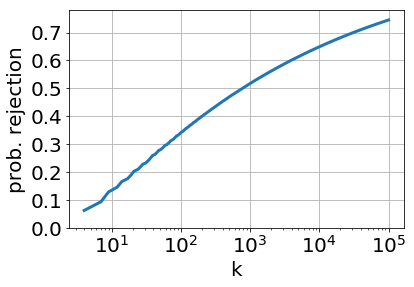
\includegraphics[width=.48\textwidth]{pics/example_plot_p05_s01.png}}\hfill
	\subfloat[\inote{Use logarithmic scale for x axis as in Figure~\ref{fig:why-adjustment-is-needed-binomial}}Need for correction in a multinomial setting. Experimental evaluation of failure probability.  \label{fig:why-adjustment-is-needed-multinomial}]{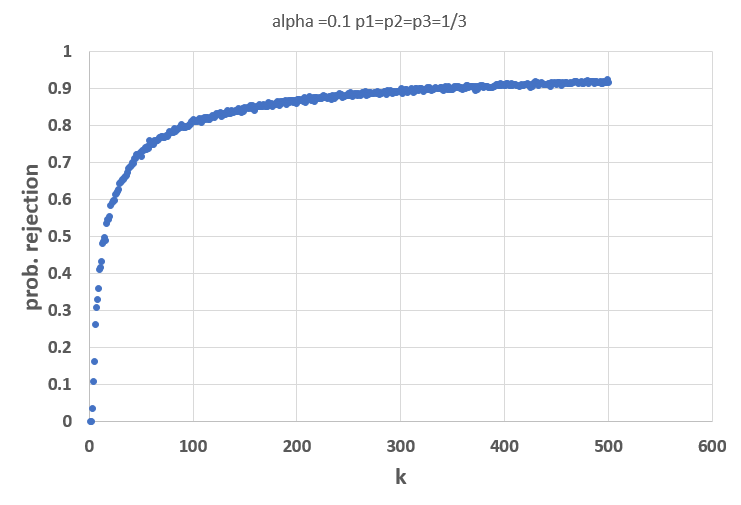
\includegraphics[width=.48\textwidth]{pics/Figure_1_Multinomial.png}}\hfill
	\caption{}
	\label{fig:need-for-model-adjustment}
	\vspace{-3mm}
\end{figure}
\todo{change figures~\ref{fig:need-for-model-adjustment} to have same appearances}

Generally, we can see that the probability of a Type-I error (declaring this fair ranking as unfair) is higher than $\alpha = 0.1$.
%
If the $k$ tests were independent, we could use $\alphaadj = 1 - (1 - \alpha)^{1/k}$ (i.e., {\v S}id{\'a}k's correction), but given the positive dependence, the false negative rate is smaller than the bound given by {\v S}id{\'a}k's correction.

We will separate the explanation of the model adjustment into two subsections: first we explain the simpler case of a binomial distribution, i.e. the presence of one non-protected and \emph{one} protected group, which can be solved analytically.
%
Second we explain the more general case of a multinomial distribution, where more than one protected group is present.

\subsubsection{Model Adjustment for One Protected Group}\label{subsubsec:adjustment-binomial}
For the binomial case we assume that a ranking generated by the process of~\citet{yang2016measuring} with parameter $p$ is inherently fair.
%
Hence our ranked group fairness test should not reject any of these rankings at a rate higher than significance level $\alpha$.
%
The probability that such a fair ranking passes the ranked group fairness test with parameters $(p,\alpha)$ can be computed as follows:
%
Let $m(k) = m_{\alpha,p}(k) = F^{-1}(k,p,\alpha)$ be the number of protected elements required up to position $k$.
%
Let $\minv(i) = k$ s.t. $m(k) = i$ be the position at which $i$ protected elements are required.
%
Let $b(i) = \minv(i) - \minv(i-1)$ (with $\minv(0) = 0$) be the size of a ``block,'' that is, the gap between one increase and the next in $m(\cdot)$.
%
An example is shown on Table~\ref{tbl:example_mtable}.
%
\begin{table}[h]
	\caption{Example of $m(\cdot)$, $\minv(\cdot)$, and $b(\cdot)$ for $p=0.5, \alpha=0.1$.}
	\vspace{-3mm}
	\label{tbl:example_mtable}
	{\small
		\begin{tabular}{cccccccccccccc}\toprule
			$k$    & 1 & 2 & 3 & {\bf 4} & 5 & 6 & {\bf 7} & 8 & {\bf 9} & 10 & 11 & {\bf 12} \\
			\midrule
			$m(k)$ & 0 & 0 & 0 & \multicolumn{1}{c|}{1} & 1 & 1 & \multicolumn{1}{c|}{2} & 2 & \multicolumn{1}{c|}{3} & 3  & 3  & \multicolumn{1}{c}{4}\\
			Inverse   & \multicolumn{4}{c|}{$\minv(1)=4$}
			& \multicolumn{3}{c|}{$\minv(2)=7$}
			& \multicolumn{2}{c|}{$\minv(3)=9$}
			& \multicolumn{3}{c}{$\minv(4)=12$}\\
			Blocks       & \multicolumn{4}{c|}{$b(1)=4$}
			& \multicolumn{3}{c|}{$b(2)=3$}
			& \multicolumn{2}{c|}{$b(3)=2$}
			& \multicolumn{3}{c}{$b(4)=3$}\\\bottomrule
		\end{tabular}
	}
\end{table}

\noindent Furthermore let
\begin{equation}
\label{eq:combinations}
I_\ell = \{ (i_1, i_2, \ldots, i_\ell): \forall \ell' \in [\ell], 0 \le i_{\ell'} \le b(\ell') \wedge \sum_{j=1}^{\ell'} i_j \ge \ell' \}
\end{equation} represent all possible ways in which a fair ranking generated by the method of \citet{yang2016measuring} can pass the ranked group fairness test up to block $\ell$, with $i_j$ corresponding to the number of protected elements in block $j \; (\text{with } 1 \le j \le k)$ where $[\ell]=\lbrace 0,1,\ldots,(\ell -1) \rbrace$.
%
The probability of considering this ranking of $k$ elements (i.e. $m(k)$ blocks) unfair, is:
\begin{equation} \label{eq:failureProb}
1 - \sum_{v \in I_{m(k)}} \prod_{j=1}^{m(k)} f(v_j; b(j), p)
\end{equation}
%
\noindent where $f(x;b(j),p) = Pr(X = x)$ is the probability density function of a binomially-distributed variable $X \sim Bin(b(j), p)$.
%
This expression however is intractable because of the large number of combinations in $I_{m(k)}$.
%
Zehlike et al. \cite{zehlike2017fair} proposed an efficient iterative method seen in algorithm \ref{alg:correction} to compute the probability that a fair ranking passes the ranked group fairness test.
%
However, this algorithm produced incorrect results for   some few sets of $(k,p,\alpha)$.
%
This is due to the fact that the algorithm does only compute the right result for full blocks.
%
If a block is \" broken in half \" because the ranking size k has been reached, the calculation was off.
%
This is why we propose algorithm \ref{alg:correction_recursive} which computes the probability that a fair ranking passes the ranked group fairness test (i.e. the right term of Equation~\ref{eq:failureProb}) recursively.
%
The algorithm breaks the vector $(i_1, i_2, \ldots ,i_{\ell})$ of equation \ref{eq:combinations} in \textit{prefix} and \textit{suffix}.
%
We call $i_1$ the \textit{prefix} of $(i_2, \ldots, i_{\ell})$, and $(i_2, \ldots, i_{\ell})$ the \textit{suffix} of $i_1$.
%
The algorithm starts with a prefix and calculates all suffixes recursively.
%
For example, for the first prefix $i_1 = 0$ the algorithm computes all possible combinations where we rank zero protected candidates in the first block.
%
In the next recursion $i_1=0, i_2 =1$ the algorithm computes all possible combinations where we rank zero protected candidates in the first block and one protected candidate in the second block.
%
Additionally the algorithm computes all possible combinations with different numbers of protected candidates per block, reaching from the minimum number of protected candidates to be ranked to the maximum.
%
Following our example this means that after all combinations for prefix $i_1 = 0$ are calculated, the algorithm computes all combinations for $i_1 = 1$.
%
In summary there are at most $\prod_{j=1}^{m(k)}b(j)$ possible combinations.
%
Note that many possible combinations of $I_{m(k)}$ share the same prefix and hence the same probability density value for these prefixes.
%
To reduce computation time the algorithm stores the binomial probability density value for each prefix in a hash map with the prefix as key and the respective PDF as value.
%
Thus the overall computational complexity becomes: $O(\prod_{j=1}^{m(k)}b(j) \cdot O(\texttt{binomPDF}))$

We use Algorithm~\ref{alg:correction_recursive} to determine the adjusted significance level $\alphaadj$ for the ranked group fairness test, such that the overall acceptance probability becomes $1-\alpha$.
%
This is done by performing a binary search on $k$-dimensional vectors $(m(1), m(2), \ldots , m(k))$ called \textit{mTables} as shown in Table~\ref{tbl:example_mtable}.
%
A $k$-dimensional vector (e.g. $(0,0,1,2,3)$) has to have two properties in order to constitute a mTable, rather than just an array of integers: it has to be \emph{valid} and \emph{legal}.
%
\begin{definition}[Valid mTable]
	\label{def:valid-mtable}
	The $\text{mTable}_{p,k,\alpha}=(m(1) , m(2) , \ldots , m(k))$ is \emph{valid} if and only if, $m(i) \leq m(j)$ for all $i,j \in \lbrace 1, \ldots, k \rbrace$ with $i < j$ and $m(i)=n \Rightarrow m(i+1) \leq n+1$.
\end{definition}
\noindent It is easy to see that many valid mTables exist.
%
They correspond to all $k$-dimensional arrays with integers monotonically increasing by array indices.
%
However we only want to consider those valid mTables that correspond to the binomial ranking procedure by~\citet{yang2016measuring} for our ranked group fairness test.
%
We call these legal mTables.
%
\begin{definition}[Legal mTable]
	\label{def:legal-mtable}
	A $\text{mTable}_{p,\alpha,k}$ is \textit{legal} if and only if there exists a $p,k,\alpha$ such that
	$\texttt{constructMTable}(p,k,\alpha)=MT$.
\end{definition}
%
\begin{definition}[constructMTable]
\label{def:construct-mtable-single-test}
For $p\in(0,1), k \in \mathbb{N}, \alpha \in [0,1]$ we define a function to construct a mTable from input parameters $p, k, \alpha$ according to the procedure by~\citet{yang2016measuring}.

\noindent$\texttt{constructMTable} :(0,1) \times \mathbb{N} \times [0,1] \longrightarrow \lbrace (m(1) ,\ldots, m(k)): m(i) = F^{-1}(i,p,\alpha) | i = 1,\ldots,k\rbrace$ with $\texttt{constructMTable}(p,k,\alpha)=\text{mTable}_{p,k,\alpha}$.
\end{definition}
%
\begin{lemma}
	\label{lemma:legal-valid-mtable}
	If a mTable is legal, it is also valid.
\end{lemma}
%
\noindent Lemma \ref{lemma:legal-valid-mtable} follows directly by construction. Again, in Algorithm~\ref{alg:correction_recursive} our goal is to find the correct $\alphaadj$ using binary search.
%
A binary search procedure is possible because for any value of $\alpha$ there exists exactly one \emph{legal} mTable.
%
However, the opposite is not true: as $\alpha$ is a real number from the interval $[0, 1]$, the same mTable can be created using different (but similar) values of $\alpha$.
%
Thus without a discrete measure for a mTable we do not know when to stop searching.
%
\begin{definition}[Mass of a mTable]
\label{def:Mass of a MTable}
For $\text{mTable}_{p,k,\alpha}=(m(1) , m(2) , \ldots , m(k))$ we call\\
$L_1(\text{mTable}_{p,k,\alpha})=\sum_{i=1}^k m(i)$ the \textit{mass of $\text{mTable}_{p,\alpha,k}$}.
\end{definition}
\noindent This discrete measure $L_1(\text{mTable}_{p,k,\alpha})$ relates to the failure probability (Eq.~\ref{eq:failureProb})
%, i.e. the probability that a ranking created by use of $\text{mTable}_{p,k,\alpha}$ fails the ranked group fairness test,
in the following way:
\begin{lemma}
\label{lemma:non-decreasing-with-alpha-mtable}
Every $\text{mTable}_{p,k,\alpha}=\texttt{constructMTable}(p,k,\alpha)=(m(1) , m(2) , \ldots , m(k))$ is non-decreasing with $\alpha$. This means that
$\texttt{constructMTable}(p,k,\alpha - \epsilon) = (m(1)' , m(2)' , \ldots , m(k)')$ will result in $m(i)' \leq m(i)$ for $i=1,\ldots,k$ and $\epsilon > 0$.
\end{lemma}
\noindent This property shows that, if we reduce $\alpha$ in our binary search, the mass of the corresponding mTable is also reduced or stays the same.
%
It very usefully implies a criterion to stop the binary search: namely we stop the calculation when the mass of the mTable of the left search boundary equals the right search boundary.
%
Of course this only works if there exists exactly one legal mTable for each mass, which we prove in the following:
%
\begin{theorem}
\label{theorem: mtable-mass-injection}
For fix $p,k$ there exists exactly one legal mTable for each mass $L_1\in \lbrace 1,\ldots,k \rbrace$.
\end{theorem}
\begin{proof}
\label{proof: mtable-mass-injection}
Let $MT_{p,k,\alpha_1}$ and $MT'_{p,k, \alpha_2}$ be two different mTables with $L_1(MT_{p,k,\alpha_1 }) = L_1(MT'_{p,k,\alpha_2})$.\\
%
If both are legal then it applies that $\texttt{constructMTable}(p,\alpha_1 ,k)=MT_{p,\alpha_1 ,k}$
and \\ $\texttt{constructMTable}(p,\alpha_2 ,k)=MT'_{p,\alpha_2 ,k}$.
%
Because $MT_{p,k,\alpha_1} \neq MT'_{p,k,\alpha_2}$, without loss of generality entries $m(i), m(i)' , m(j) , m(j)'$ exist in each table, such that $|m(i) - m(i)'| = |m(j) - m(j)'|$ while at the same time $m(i) > m(i)'$ , $m(j) < m(j)'$ for $i<j, i,j \in \lbrace 1, \ldots , k \rbrace$.
%
(Think of it as the two entries in each table "evening out", such that both tables have the same mass.)\\
%
If $\alpha_1 > \alpha_2$, then the statement $m(j)' > m(j)$ violates Lemma~\ref{lemma:non-decreasing-with-alpha-mtable}.
%
If $\alpha_2 > \alpha_1$, then the statement $m(i) > m(i)'$ also violates Lemma~\ref{lemma:non-decreasing-with-alpha-mtable}.
%
The only possibility left is hence that $\alpha_1 = \alpha_2$, which contradicts $MT \neq MT'$, as both are created using function \texttt{constructMTable}.
\end{proof}

In order to estimate the complexity of the whole procedure (and hence understand its computational feasibility), we need to know how many mTables exist for fix $k$ and $p$.
%
The pseudo code of the algorithm is shown in the appendix of this paper (see Algorithm~\ref{alg:binom_binary}.)
\begin{theorem}
\label{theorem:number-of-mtables}
The number of legal mTables for $k,p$ is less or equal to $\frac{k(k-1)}{2}$ .
\end{theorem}

\begin{proof}
\label{proof:number-of-mtables}
With the proof above we can count the number of legal mTables for fix $p,k$ as follows: The maximum mass of a legal mTable of length $k$ is by construction
$L_1 ((m(1) = 1,m(2) = 2, \ldots, m(k) = k)) = \sum_{i=1}^k m(i) = \frac{k(k-1)}{2}$
%
Following definition~\ref{def:valid-mtable} the entry $m(1)$ is either $0$ or $1$.
%
In turn $m(2)$ can only be $2$, if $m(1)$ was $1$ (otherwise $m(2)<2$).
%
Accordingly, the minimum mass of a legal mTable is $L_1((m(1),m(2), \ldots, m(k))) = 0$, if all $m(i)=0$.
%
We have shown that exactly one legal mTable exists for each mass.
%
It follows directly that there are at most $\frac{k(k-1)}{2}$ masses and therewith legal mTables.
\end{proof}

\begin{algorithm}[t!]
	\caption{Algorithm \algoRecursive computes the probability, that a given mTable accepts a fair ranking.}
	\label{alg:correction_recursive} % But whenever possible refer to this algo. by name not number
	\small
	\AlgInput{$\texttt{b[]}$ list of block lengths (table \ref{tbl:example_mtable}), $\texttt{maxProtected}$ the sum of all entries of $\texttt{b[]}$; $\texttt{currentBlockIndex}$ index of the current block; $\texttt{candidatesAssigned}$ number of candidates assigned for the current possible solution; $p$, the expected proportion of protected elements.}
	\AlgOutput{The probability of accepting a fair ranking.}

	\If{$\texttt{b[].length} = 0$}{
		\Return{$1$}
	}
	\tcp{we need to assign at least one protected candidate each block}
	$\texttt{minNeededThisBlock} \leftarrow \texttt{currentBlockIndex} - \texttt{candidatesAssigned}$\\
	\tcp{if we already assigned enough candidates, minNeededThisBlock = 0}
	\If{$\texttt{minNeededThisBlock} < 0$}{
		$\texttt{minNeededThisBlock} \leftarrow 0$
	}
	$\texttt{maxPossibleThisBlock} \leftarrow \textit{argmin}(\texttt{b[0]}, \texttt{maxProtected})$ \\
	$\texttt{assignments} \leftarrow 0$ \\
	$\texttt{successProb} \leftarrow 0$ \\
	$\texttt{b\_new[]} \leftarrow \textit{sublist}(\texttt{b[]}, 1, \texttt{b[].length})$ \tcp*{sublist without the first entry of $\texttt{b[]}$}
	\While{$\texttt{itemsThisBlock} \leftarrow \texttt{minNeededThisBlock} \leq \texttt{maxPossibleThisBlock}$}{
		$\texttt{remainingCandidates} \leftarrow \texttt{maxProtected} - \texttt{itemsThisBlock}$ \\
		$\texttt{candidatesAssigned} \leftarrow \texttt{candidatesAssigned} + \texttt{itemsThisBlock}$ \\
		\tcp{the suffixes are the success probabilities of all possible ways to fairly rank protected candidates after this block}
		$\texttt{suffixes} \leftarrow \textsc{\algoRecursive}(\texttt{remainingCandidates}, \texttt{b\_new[]}, \texttt{currentBlockIndex} + 1, \texttt{candidatesAssigned})$ \\
		$\texttt{successProb} \leftarrow \texttt{successProb} + \textsc{BinomPMF}(\texttt{maxPossibleThisBlock}, \texttt{itemsThisBlock}, p) \cdot \texttt{suffixes}$ \\
	}
	\Return{probability of accepting a fair ranking: $\texttt{successProb}$ }
\end{algorithm}

\subsubsection{Model Adjustment for Multiple Protected Groups}
\label{sec:multinomial-adjustment}
%
With the presence of more than one protected group, the analytical extension of the model adjustment to a multinomial setting is too complex to be written into a closed formula.

We found no efficient way to calculate all permutations which pass or fail the test and we choose an experimental procedure to adjust $ \alpha $.
%
It is a generalization of the binomial process suggested by~\citet{yang2016measuring} to multinomial settings:
\begin{enumerate}
	\item Get input $ p_G, k, \alpha $.
	\item Build mTree with input $ \alpha $.
	\item Create $M$ rankings by rolling a biased $ |G| $-sided dice with each side's probability to show corresponding to a minimum proportion in vector $ p_G $.
	\item Test all those rankings against the mTree and count how many tests fail.
	%
	Remember that we want to observe a maximum failure probability of $ \failprob=\alpha $, because all rankings created by this multinomial stochastic process are considered to be inherently fair.
	\item If $ \failprob \neq \alpha $, we choose a new $ \alphaadj $ using a binary search heuristic.
	\item Now we build a new mTree using $ \alphaadj $ and repeat the procedure until $ \failprob \approx \alpha $.
\end{enumerate}
%
This adjustment procedure requires to compute a new mTree at each iteration which is expensive on its own. Depending on the level of accuracy needed, a large number of iterations $M$ might be required.
%
Additionally the binary search heuristic needs many steps to find $\alpha$, if large intervals have to be searched.

We use three strategies to drastically reduce computational costs.
%
\begin{inparaenum}[(1)]
%
\item we reduce the space requirements of the mTree structure;
%
\item we construct the tree level by level and reject if the ranking does not satisfy any node in a level;
%
\item we exploit the monotonicity of $\alphaadj$ with respect to $\alpha$ and use a regression procedure to speed up the binary search.
\end{inparaenum}
%
We next explain each strategy.


First, we improve the mTree data structure itself by excluding the calculation and storage of redundant information.
%
Figures~\ref{fig:mtree-symmetric-adjusted} and~\ref{fig:mtree-asymmetric-adjusted} show the mTree structure with all parent-child relations as edges.
%
In these structures, a node can only appear once at each level. Duplicate nodes are combined into a single node with multiple parents.
%
Furthermore we reduce the size of the mTree by actually leaving out the parent-child relationship and merely storing the nodes itself together with their respective depth levels.
%
This is possible because we know that, if a single node exists on each level, which accepts a given ranking as fair, then a valid path to that node exists in the tree.
%
Before we can prove this property, we need to introduce the following definition.
%
\begin{definition}[Successful mTree Testing]
\label{def:valid-mtree-test}
Let $\tau$ be a ranking of size $k$ and $\tau_{G,i}=(\tau_{1},\ldots,\tau_{|G|})$ the numbers of ranked protected elements from group $1,\ldots,|G|$ up to position $i$.
%
Let furthermore $MT$ be a $mTree$, with $MT_{G,i}=[m_1(i),\ldots,m_{|G|}(i)]$ the number of protected candidates of group $1,\ldots,|G|$ required up to position $i$.
%
We write $\tau_{G,i} \geq m_{G,i}$ if $\tau_g \geq m_g$ for all $g=1,\ldots,|G|$.
%
We call a test on level $i$ of $MT$ successful if and only if $\tau_{G,i} \geq m_{G,i}$.
\end{definition}
%
\noindent With this we can make sure that if we test a ranking on each level of the mTree successfully, the entire ranking will be fair according to the ranked group fairness definition.
%
We prove this by showing that, if a ranking passes the test for any two nodes $n_1$ and $n_2$ at two consecutive levels $h$ and $h+1$ and $n_1$ is \emph{not} a parent of $n_2$, then all actual children of $n_1$ will have a weaker requirement than $n_2$ and will hence also test successfully.
%
Furthermore we show that all nodes at level $h+1$ for which the ranking fails the test are part of a path that already rejected it as unfair at level $h$.
%
Consider an example from Figure~\ref{fig:mtree-symmetric-adjusted} : Let us assume a ranking passes the test at level $9$ with exactly the required protected items $[1,1]$.
%
Now lets assume that at level $10$, the given ranking would pass the test for node $[2,1]$, which is not a successor of $[1,1]$.
%
In fact we see that the actual successor of $[1,1]$ is a node with the same configuration $[1,1]$.
%
However, if our ranking passes the test for the stricter node $[2,1]$, it also passes for $[1,1]$ and thus we do not need to know the true parent of $[2,1]$.
%
Note that the ranking would fail at node $[3,0]$, but with $[1,1]$ at level 9 it would have failed already at $[3,0]$'s predecessor $[2,0]$.
\note[ChaTo]{I did not review the following proof.}
%
\begin{theorem}
\label{theorem:lazy-mTree-test}
Let $MT$ be a mTree and $\tau$ a ranking of size $k$. If and only if there exists at least one successful test for $\tau$ at each level of $MT$, there exists a valid path from the root of $MT$ to a leaf of $MT$.
\end{theorem}
%
\begin{proof}
	\label{proof:lazy-mTree-test}
	It is clear that at least one successful test per level is necessary for the path to exist, let us prove that it is sufficient.
	%
	Let $MT$ be a mTree and $\tau$ be a ranking that passes the test at level $h$ of $MT$.
	%
	Let $m_{G,h}=[m_{1}(h), \ldots, m_{|G|}(h)]$ be the node on level $h$ that successfully tested $\tau$.
	%
	Let further be $\tau_g(h)$ the number of protected candidates of group $g$ ranked at up to position $h$.
	%
	Without loss of generality let $\sum_{g=1}^{|G|} |m_{g}(h) - \tau_{g}(h)| = 0$, meaning that the ranking includes the exact amount of required protected candidates at level $h$ and not more.
	%
	Let $m_{G,(h+1)}$ be a node which tests $\tau$ successfully on level $h+1$ with $\sum_{g=1}^{|G|} |m_{g}(h+1) - \tau_{g}(h+1)| = 0$.
	%
	For all entries $m_{g}(h+1)$ of $m_{G,(h+1)}$ it is that $m_{g}(h) \leq m_{g}(h+1)$ by construction of the mTree in which requirements for protected candidates can only increase or stay the same.

	\noindent We can now distinguish between the following two cases:
	\\
	\textbf{Case 1:} $m_{G,(h+1)}$ is a child of $m_{G,h}$.
	%
	Then they form a path. %UNNECESSARY:% Note that $\sum_{g=1}^{|G|} (m_{g}(h+1) - m_{g}(h) \leq 1)$.
	\\
	\textbf{Case 2:} $m_{G,(h+1)}$ is not a child of $m_{G,h}$.
	%
	Let now ${m'}_{G,(h+1)}$ be a child of $m_{G,(h)}$.
	%
	Because of $\sum_{g=1}^{|G|} |m_{g}(h) - \tau_{g}(h)| = 0$, and a successful test at level $h+1$, the following inequations hold: $\sum_{g=1}^{|G|} |m_{g}(h) - m_g(h+1)| \leq 1$ and $\sum_{g=1}^{|G|} |m_{g}(h) - m'_g(h+1)| \leq 1$.
	%
	If $\sum_{g=1}^{|G|} |m_{g}(h) - m_g(h+1)| = \sum_{g=1}^{|G|} |m_{g}(h) - m'_g(h+1)| = 0$ or $\sum_{g=1}^{|G|} |m_{g}(h) - m_g(h+1)| = \sum_{g=1}^{|G|} |m_{g}(h) - m'_g(h+1)| = 1$, it follows that $m_{G,(h+1)} = {m'}_{G,(h+1)}$ and we would have a contradiction with the fact that ${m'}_{G,(h+1)}$ is not a child of $m_{G,h}$, because then the nodes would be equal or different by one unit in one position.

	Hence, we need that either
	(2.1) $\sum_{g=1}^{|G|} |m_{g}(h) - m_g(h+1)| = 1$ and $\sum_{g=1}^{|G|} |m_{g}(h) - m'_g(h+1)| = 0$,
	or
	(2.2) $\sum_{g=1}^{|G|} |m_{g}(h) - m_g(h+1)| = 0$ and $\sum_{g=1}^{|G|} |m_{g}(h) - m'_g(h+1)| = 1$.
	%
	Case (2.1) means because of $\sum_{g=1}^{|G|} |m_{g}(h) - m_g(h+1)| = 1 < \sum_{g=1}^{|G|} |m_{g}(h) - m'_g(h+1)| = 0$ that the mTree accepts a ranking with one more protected candidate than required by the actual child of $m_{G,h}$, which contradicts our hypothesis that the ranking included the exact amount of required protected candidates. It follows that if we test $\tau_g (h+1)$ successfully with $m_{G,h+1}$ it would also satisfy ${m'}_{G,h+1}$.
Case (2.2) is impossible according to algorithm \ref{alg:imcdf}.
In detail, if $\sum_{g=1}^{|G|} |m_{g}(h) - m_g(h+1)| = 0$ it means that $ m_g(h+1) = m_{g}(h)$ and therefore, $F(m_{g}(h);h+1,p_G) > \alpha$ (line $4$ of algorithm \ref{alg:imcdf}). But if for the child of $m_{G,h}$, namely ${m'}_{G,h+1}$ it holds that $\sum_{g=1}^{|G|} |m_{g}(h) - m'_g(h+1)| = 1$, it means that
$F(m_{g}(h);h+1,p_G) \leq \alpha$ so that we would have added a new node as a child of $m_{g}(h)$ according to lines  $8-14$ of algorithm \ref{alg:imcdf}. Since both conditions cannot be true at the same time, Case (2.2) can not occur.
\\
In summary, Case (2.1) will only occur if we ranked more protected candidates than needed, and that the resulting test would be more strict than following a path through the mTree.
%
We showed that Case (2.2) is impossible. There is only Case 1 left if we have ranked exactly the number of protected candidates needed at each level of the mTree.
%
It follows that for any ranking that is tested successfully on each level of the mTree, it either was tested by nodes of a path through the mTree or was tested by a series of nodes which is more strict than such path.
\end{proof}
%
\noindent Because of theorem \ref{theorem:lazy-mTree-test} we do not need to keep the tree structure and may store only a list of tuples for each level, additionally to removing duplicate entries.
%
In case of symmetric minimum proportions $p_G$, we can further save memory and computation time, by reducing mirrored entries such as $[0,2]$ and $[2,0]$.
%
We simply flag a node for which a mirror exists on the same depth level and do not calculate the mirrored branch.

Second, we use the fact that given a value of $\alpha$, the mTree calculation is not dependent on $ k $, i.e. a mTree for $k=20$ and a mTree for $k=10$ for the same $\alpha$ are congruent within the first ten positions.
%
This means that we can start the adjustment from the root node and expand the tree gradually to find the correct $ \alphaadj $, because if $\failprob$ is too high for $k=10$ it will be too high for $k=20$ in particular and we do not have to consider the larger tree, as long as we do not have a good $\alphaadj$ for $k=10$.
%
%In order to show that we can indeed do that, assume that the for loop of algorithm \ref{alg:computeMTree} stops at $k=10$ instead of $k=20$.
%
%Furthermore, we can understand the mTree as a set of rules that a ranking has to satisfy.
%
%If there are no rules for how many protected candidates are required after position $10$, this is equivalent to not requiring more protected candidates after position $10$.
%
%Thus, the probability that a fair ranking is rejected by a shorter mTree is less or equal to a deeper mTree.
%
%We utilize this property to lower computational costs: we calculate the mTree for $k=10$, then create 10000 rankings of length 10 and calculate $ \alphaadj $ under this setting.
%
%Then we set $ k=k+ $\texttt{stepsize}, and repeat the procedure until we reach the desired ranking length.
%
We can see in Figure \ref{fig:need-for-model-adjustment} that $ \failprob $ grows very fast for small $k$, which makes an early adjustment of $\alpha$ most efficient to save computation time.

Third, we use a second-degree polynomial regression model to get our first estimate for a good $\alphaadj$ candidate and apply the binary search heuristic from that candidate, rather than starting with a random value, that might be very far away from the correct $\alphaadj$.
%
In this case we give as input a few additional parameters: \texttt{kTarget} -- the length of the target ranking, \texttt{kStart} -- the size of the first mTree, \texttt{maxPreAdjustK} -- the maximum size of the mTree before we use regression to predict a good candidate $\alpha_{c_r}$ for the final $\alphaadj$, and \texttt{num\_iterations} -- the number of training instances to be computed.
%
To create a training dataset $R$, we compute \texttt{num\_iterations} small mTrees (i.e. with different $k \leq $ \texttt{maxPreAdjustK}) and adjust the respective $\alpha$ values as described in the beginning of Section~\ref{sec:multinomial-adjustment}.
%
For each iteration $j$ the pair $(k_j, \alpha_{c_j})$ is stored as a training instance in $R$.
%
\begin{figure}[h]
	\centering
	%
	\subfloat[Training data $R$ for a linear regression model to predict a good candidate for $\alphaadj$. Each pair $(k_j, \alpha_{c_j})$ is computed for small $k$ using the procedure described in the beginning of Section~\ref{sec:multinomial-adjustment}. \label{fig:regression-training-data}]
	{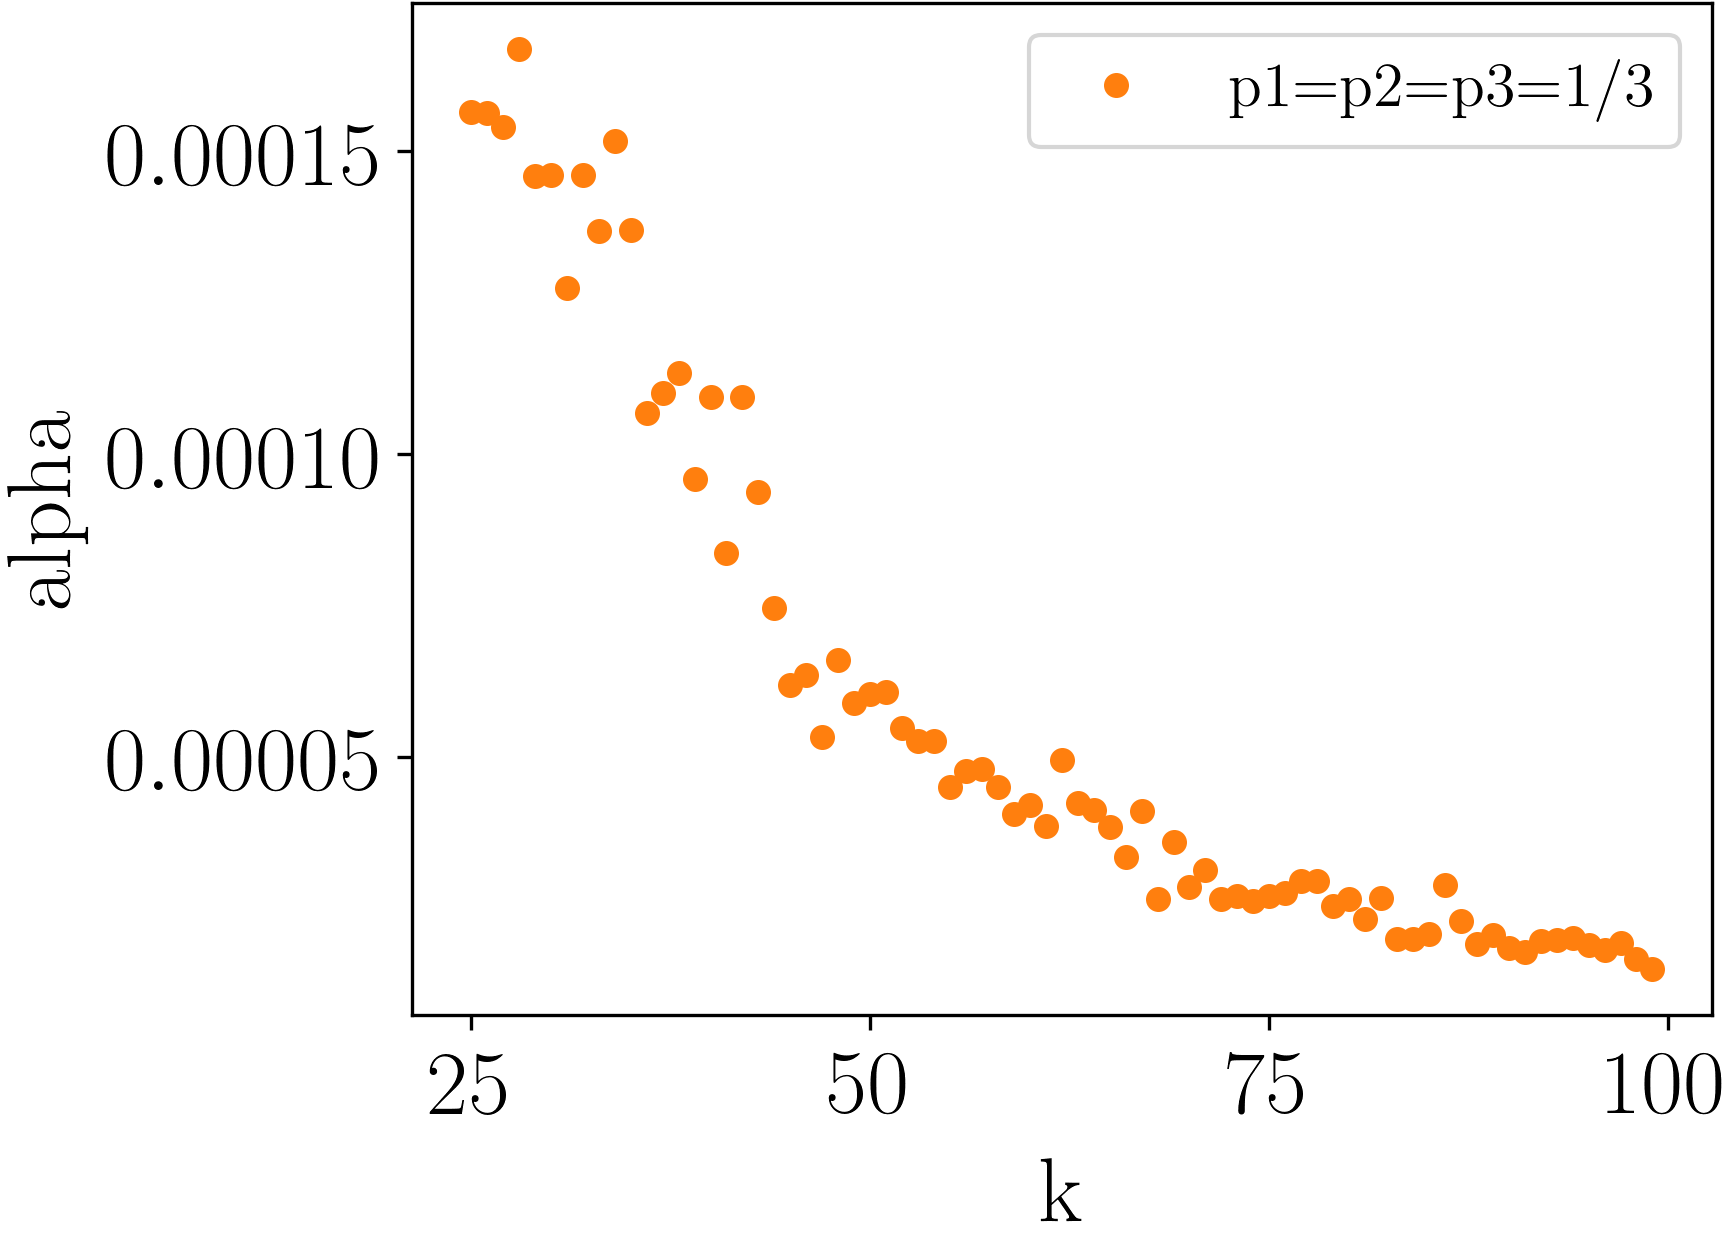
\includegraphics[width=.48\textwidth]{pics/alpha_030303_01.png}}\hfill
	%
	\subfloat[Computation time comparison between binary search only and binary search combined with linear regression for the multinomial significance adjustment.  \label{fig:regression-time-saved}]
	{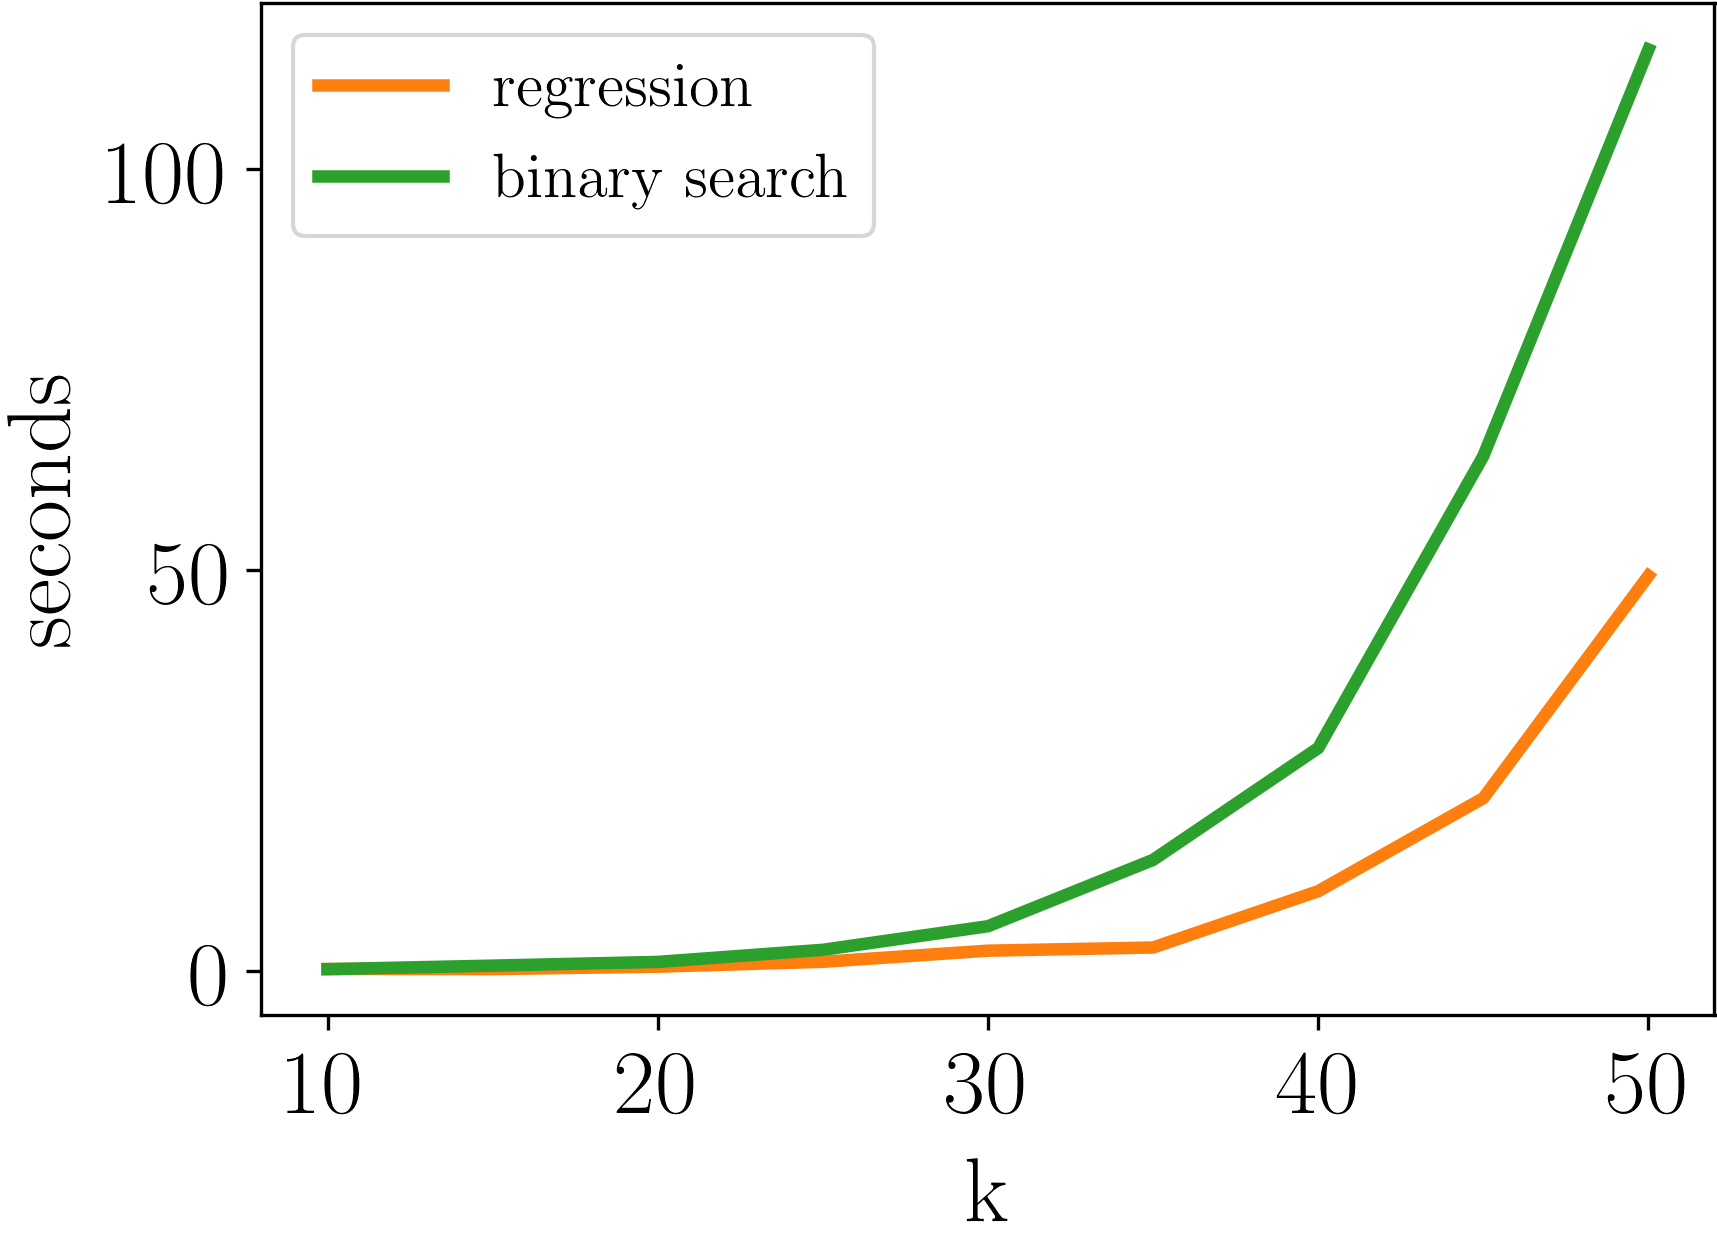
\includegraphics[width=.48\textwidth]{pics/computationTimeRegressionVSBinaryMultinomial.png}}\hfill
	\caption{}
	\label{fig:regression_adjustment_benefits}
	\vspace{-3mm}
\end{figure}
%
Figure~\ref{fig:regression-training-data} shows a training set for $p_G=[1/3, 1/3], \texttt{maxPreAdjustK}=100$.
%
Then a regression model is trained to predict $\alpha_{c_r}$ for \texttt{kTarget}.
%
This $\alpha_{c_r}$ is now used to start the binary search for the correct and final $\alphaadj$.
%
Figure~\ref{fig:regression-time-saved} shows the runtime difference for the model adjustment routine with and without the use of linear regression.

Algorithm~\ref{alg:regression_search} shows the overall adjustment procedure in pseudo-code and performs the following steps:
%
\begin{enumerate}
	\item Define the necessary parameters: \texttt{kTarget}, \texttt{kStart}, \texttt{maxPreAdjustK}, and \texttt{num\_iterations}
	\item Adjust $\alpha$ for a mTree of size \texttt{kStart} to get $\alpha_{c_1}$ using binary search.
	\item Add pair $\left(\texttt{kStart}, \alpha_{c_1}\right)$ to a regression training set $R$.
	\item \label{stepBegin} Increase $\texttt{kStart}$ by $\texttt{stepsize}=\frac{\texttt{maxPreAdjustK}}{\texttt{num\_iterations}}$
	\item Compute a mTree with parameters $\texttt{kTarget}, p_G, \alpha_{c_1}$ and adjust $\alpha_{c_1}$.
	\item \label{stepEnd} Name result $\alpha_{c_2}$ and add pair $\left(\texttt{kStart}, \alpha_{c_2}\right)$ to $R$.
	\item Repeat steps (\ref{stepBegin}) -- (\ref{stepEnd}) until $\texttt{kStart} == \texttt{maxPreAdjustK}$.
	\item Train a regression model with training data $R$ to predict $\alpha_{c_r}$ for $\texttt{kTarget}$.
	\item Use binary search (Algorithm~\ref{alg:mult_binary}) to find $\alphaadj$ for parameters $k,p_G, \alpha_{c_r}$.
\end{enumerate}
\begin{algorithm}[t!]
	\caption{Algorithm \algoReg estimates the corrected significance level $\alphaadj$ such that the mTree $m(\alphaadj , k, p_G)$ has the probability of rejecting a fair ranking $\alpha$}
	\label{alg:regression_search} % But whenever possible refer to this algo. by name not number
	\small
	\AlgInput{\texttt{kStart} -- depth of the mTree to start with; $k$ -- the length of the ranking; $p_G$ -- the desired proportions of the protected groups; $\alpha$ -- the desired significance level;  \texttt{maxPreAdjustK} the maximum depth of the mTrees that are used as training data; \texttt{num\_iterations} -- the number of steps between \texttt{kStart} and \texttt{maxPreAdjustK}}
	\AlgOutput{$\alphaadj$ -- the adjusted significance}
	$R \leftarrow \lbrace \rbrace; \alpha_{\textit{new}} \leftarrow \alpha$	\\
	\AlgComment{divide the interval [$\text{kStart}, \text{maxPreAdjustK}$] into num\_iterations parts}
	$\texttt{stepsize} \leftarrow \max(\frac{\texttt{maxPreAdjustK}}{\texttt{num\_iterations}}, 1)$ \\
	\For{$i\leftarrow 0$ to $\texttt{num\_iterations}$}{
		\AlgComment{adjust $\alpha_{\text{new}}$ for the current kStart}
    	$\alpha_{\text{new}} \leftarrow \textsc{MultinomialBinarySearchAdjustment}(\alpha_{\textit{new}}, \texttt{kStart}, p_G)$ \\
    	\AlgComment{add the pair (kStart, $\alpha_{\textit{new}}$) to the training data $R$}
    	$R.\textit{put}(\texttt{kStart},\alpha_{\textit{new}})$ \\
    	\If{$\texttt{kStart} + \texttt{stepsize} \leq \texttt{maxPreAdjustK}$}{
    		$\texttt{kStart} \leftarrow \texttt{kStart} + \texttt{stepsize}$ \\
    	}\Else{
			break
    	}
    }
    $\texttt{coeffs} \leftarrow R.\textit{train}()$ \AlgComment{returns the vector of predicted coefficients for the curve over $R$}
    $\alpha_{c_r} \leftarrow \texttt{coeffs[0]} + \texttt{coeffs[1]} * k + \texttt{coeffs[2]} * k^2$ \\
    $\alphaadj \leftarrow \textsc{MultinomialBinarySearchAdjustment}(\alpha_{c_r},k,p_G)$ \\
   \Return{$\alphaadj$}

\end{algorithm}
%
Once we found $\alphaadj$ we can recompute the mTrees from  Figures~\ref{fig:mtree-symmetric-unadjusted} and~\ref{fig:mtree-asymmetric-unadjusted} to obtain an overall significance level of $\alpha$.
%
Figures~\ref{fig:mtree-symmetric-adjusted} and~\ref{fig:mtree-asymmetric-adjusted} show the adjusted mTrees with the same parameters $p_G$.
\begin{figure}[h]
	\centering
	\begin{forest}
		for tree={
			child anchor=west,
			parent anchor=east,
			grow'=east,
			draw,
			anchor=west,
		}
		[{[0, 0]}
		[{[0, 0]}
		[{[0, 0]}
		[{[0, 0]} 
		[{[0, 0]}
			[{[1, 0]}
			[{[1, 0]}
				[{[2, 0]}
				[{[2, 0]}
					[{[3, 0]}]
					[{[2, 1]}]
				]]
				[{[1, 1]}, name=doubled1
				[{[1, 1]}
				[{[1, 1]}
				]]]
			]]
			[{[0, 1]}
			[{[0, 1]}, name=parentDoubled1
				[{[0, 2]}
				[{[0, 2]}
					[{[1, 2]}]
					[{[0, 3]}]
				]]
			]]
		]]]]]]
		\draw (parentDoubled1.east)--(doubled1.west);
	\end{forest}
	\CaptionMargin
	\caption{Example of an mTree with two protected groups with minimum proportions $ p_G=[1/3, 1/3] $ and $ \alphaadj=0.1 $. Compared to figure~\ref{fig:mtree-symmetric-unadjusted} this tree is less strict such that its \emph{total} probability $ \alphaadj $ of rejecting a fair ranking (i.e. a type-1-error) is 0.1.
	\label{fig:mtree-symmetric-adjusted}}
	\tablemargin
\end{figure}

\begin{figure}[h]
	\centering
	\begin{forest}
		for tree={
			child anchor=west,
			parent anchor=east,
			grow'=east,
			draw,
			anchor=west,
		}
		[{[0, 0]}
			[{[0, 0]}
				[{[0, 0]}
					[{[1, 0]}
						[{[1, 0]}
							[{[2, 0]}
								[{[2, 1]}
									[{[2, 1]}, name=doubled2, before drawing tree={y-=1em}
										[{[2, 1]}, before drawing tree={y-=1em}
											[{[3, 1]}, before drawing tree={y-=1em}]
											[{[2, 2]}, before drawing tree={y-=1em}]
										]
									]
								]
							]
							[{[1, 1]}, name=doubled1
								[{[1, 1]}, name=parentDoubled2
									[{[1, 2]}, name=doubled3, before drawing tree={y-=1em}
										[{[1, 2]}, before drawing tree={y-=1em}
											[{[1, 2]}, before drawing tree={y-=1em}]
										]
									]
								]
							]
						]]							
					[{[0, 1]}
						[{[0, 1]}, name=parentDoubled1
							[{[0, 2]}
								[{[0, 2]}, name=parentDoubled3
									[{[0, 3]}, before drawing tree={y-=1em}
										[{[0, 3]}, before drawing tree={y-=1em}
											[{[1, 3]}, before drawing tree={y-=1em}]
											[{[0, 4]}, before drawing tree={y-=1em}]
										]
									]
								]
							]
						]]
					]]]
		\draw (parentDoubled1.east)--(doubled1.west);
		\draw (parentDoubled2.east)--(doubled2.west);
		\draw (parentDoubled3.east)--(doubled3.west);
	\end{forest}
	\CaptionMargin
	\caption{Example of an mTree with two protected groups with minimum proportions $ p_G=[0.2, 0.4] $ and a corrected $ \alpha_c=0.1 $. 
	%
	The tree is less strict than the mTree in Figure~\ref{fig:mtree-asymmetric-unadjusted}.
	%
	The adjusted tree yields an overall false-negative rate of $ \alpha_c=0.1 $ when testing rankings for ranked group fairness.
	\label{fig:mtree-asymmetric-adjusted}}
	\tablemargin
\end{figure}

\FloatBarrier
